\documentclass[11pt,twocolumn]{article}
\usepackage[margin=0.8in]{geometry}                % See geometry.pdf to learn the layout options. There are lots.
\geometry{letterpaper}                   % ... or a4paper or a5paper or ... 
%\geometry{landscape}                % Activate for for rotated page geometry
%\usepackage[parfill]{parskip}    % Activate to begin paragraphs with an empty line rather than an indent
\usepackage[breaklinks=true, colorlinks=true, linkcolor=red, urlcolor=blue, citecolor=black]{hyperref}
\urlstyle{rm}
\usepackage{amsmath}
\usepackage{mathptmx}
\usepackage{graphicx}
\usepackage{amssymb}
\usepackage{epstopdf}
\usepackage{color}
\usepackage{sidecap}
\usepackage{authblk}
\usepackage{booktabs}
\usepackage[font=small,labelfont=bf]{caption}
\DeclareGraphicsRule{.tif}{png}{.png}{`convert #1 `dirname #1`/`basename #1 .tif`.png}
\usepackage{enumitem}
\setlist[itemize]{noitemsep}
\setlist[enumerate]{noitemsep}

\def\bfr{\bf\color{red}}
\def\geohub{{\tt geohub}}
\def\Count{count}
\def\ntracts{39}
\def\nprof{9}
\def\nvol{30}
\def\resp{respectively}

\title{\bf
	Results of the 2021 Volunteer Greater Hollywood Homeless Count
	}
\author[*,$\dagger$,$\ddagger$]{Louis Abramson, PhD}%,$\ddagger$
\affil[*]{\it Hollywood 4WRD Homelessness Coalition, 6255 Sunset Blvd, Ste 150, LA, CA 90028}
\affil[$\dagger$]{\it Central Hollywood Neighborhood Council, PO Box 93907, LA, CA 90093}
\affil[$\ddagger$]{\it Carnegie Observatories, 813 Santa Barbara St, Pasadena, CA 91101}
\affil[ ]{\href{mailto:labramson.chnc@gmail.com}{labramson.chnc@gmail.com}}
%\affil[$\dagger$]{\it Princeton University, 4 Ivy Lane, Princeton, NJ 08544}
%\href{mailto:labramson.chnc@gmail.com}{labramson.chnc@gmail.com}}

\date{\today}                                           % Activate to display a given date or no date

\begin{document}
\maketitle

\begin{abstract}

The Los Angeles Homelessness Services Authority (LAHSA) opted not to sponsor a 2021 Unsheltered 
Point In Time Count. Despite this, service providers, business leaders, residents, and other organizations
in Hollywood decided to proceed with an analogous if unsponsored event on 25 February 2021. XXX 
volunteer vehicle-based teams and YYY professional foot outreach teams performed visual inspections of
all 39 US Census tracts in the official Hollywood and East Hollywood Continua of Care (CoCs). Based on 
the 2020 official LAHSA dwelling weighting factors, we estimate that there are $xxx\pm yyy$ unsheltered 
people living on the streets of those CoCs (90\% confidence). Modulating the weights leads to variability
of XXX. We conclude that YYY. All data and results are presented in tabular form, with materials, and
analysis code presented in the Appendix or on request.

\end{abstract}

\section{Introduction}
\label{sec:intro}

The Los Angeles Homelessness Services Authority (LAHSA) has conducted an annual Point In Time (PIT) 
census of the unhoused population of Los Angeles County every year since 20{\bfr XX}. These data are critical to 
essentially all homelessness-related activities in the County and its municipalities. They inform programmatic
funding levels, educate residents, undergird local and state legislative efforts, and shape the day-to-day 
practices of thousands of professional and volunteer service providers. As the official assessment of the 
scope of one of the most pressing humanitarian issues of our time, the LAHSA Count is invaluable.

Disruptions from COVID-19 have both challenged and re-emphasized the need for such data. As incomes 
have fluctuated, Los Angeles' already sizable community of housing-unstable residents have only grown more
at risk of being pushed off couches or out of apartments and onto the street. As such, while the 
epidemiological considerations related to an all-volunteer countywide census are real, the potential 
damage from failing to conduct one so is also substantial.

Given the non-uniformity in volunteerism and resources across LAHSA's large area of operations, 
the challenges of COVID were ultimately deemed sufficient to cancel the formal 2021 PIT census of 
unsheltered Angelenos. However, not all communities agreed with that decision. Hollywood was one 
such community.

Greater Hollywood is an epicenter of LA's homelessness crisis. According to the official 2020 
Count, the Hollywood and East Hollywood Continua of Care (CoC) were home to 2203 unhoused residents,
1714 of whom (78\%) were living unsheltered on the street. This figure corresponds to roughly 5\% of LA's 
homeless population concentrated in an area with only 2.5\% ({\bfr CITE}) of its total population. In some 
regions in those CoCs, 1-in-30 residents are unhoused compared to 1-in-100 citywide.

While the above statistics are tragic, Hollywood is also marked by increasingly formal coalitions of 
service providers, business leaders, residents, and quasi-governmental entities dedicated to humanely 
ending the homelessness crisis. Each of these stakeholders relies on the annual PIT count: lay residents need
to be educated as to the size of the challenge; funders need to understand how many people require services;
legislators need to know how many people are dwelling where. For these reasons, and given the 
capacity of the above organizations and individuals, the Hollywood community decided to proceed with 
an unsponsored 2021 PIT \Count.

This document describes the methodology and findings of that \Count, which took place on the night of 
Thursday, February 25, 2021. Section \ref{sec:procedure} describes data acquisition, analysis, and volunteer
training protocols. Section \ref{sec:results} present estimates of the unsheltered 
populations in the Hollywood and East Hollywood CoCs. Section \ref{sec:discussion}
contextualizes those findings in terms of previous LAHSA results and describes factors that would
modulate them upwards or downwards. Section \ref{sec:summary} summarizes. Additional information
can be found in the Appendix, including a table of tract-level results in each of the survey's 39 US 
Census tracts.

\section{Methodology}
\label{sec:procedure}

Our \Count\ took place on 25 February 2021 beginning at 7.00 PM. This date and time correspond to 
roughly one month later and four hours earlier than the official event would have occurred. Beyond
those choices, our program adhered as closely as possible to the official LAHSA 2020 PIT data 
collection and analysis protocols. Ancillary data from regularly monitored census tracts suggests 
that the date offset is unlikely to substantially erode comparability between this and past datasets, 
though {\bfr we have less purchase on time-of-day effects}.

The \Count\ was based out of The Center at Blessed Sacrament (``The Center''), a major service 
provider in Hollywood, at 6636 Selma Ave. All volunteer teams launched from and returned to this 
location as they would in previous years to a LAHSA community count hub. The major difference 
was that training was performed remotely as a COVID precaution, and volunteer counters never left 
their vehicles.

\subsection{Data Acquisition}
\label{sec:acquisition}

The \Count\ covered the \ntracts\ US Census tracts constituting the LAHSA-defined Hollywood 
and East Hollywood Continua of Care (CoC; 21 and 18 tracts, \resp). Our \Count\ did not recognize census 
tract ``splits'' or sub-tracts---e.g., ``1905.10a''---which sets a coarser resolution floor to our results 
compared to past PIT results. That choice also slightly modifies of the definition of the Hollywood CoC 
to include all of tract 1905.10 as opposed to only the ``a'' sub-tract. Such a modification has a negligible 
impact on CoC-level results (since 2016, split 1905.10b has never been seen to host more than 7 unsheltered 
people). Sections \ref{sec:results} and \ref{sec:discussion} discuss CoC results with tract-level tallies provided
in the Appendix. Results for Greater Hollywood are not directly comparable to any official service 
geography, but are available upon request for educational purposes. Figure \ref{fig:map} shows 
the \Count\ footprint.

\begin{figure*}
	\centering
	\includegraphics[width=0.9\linewidth]{map}
	\caption{The 2021 volunteer \Count\ covered Greater Hollywood, comprising the 
			officially recognized LAHSA Hollywood and East Hollywood Continua
			of Care. The former stretches from Laurel Canyon Blvd to Western Ave,
			the latter from Western to Hoover Ave. Hollywood is bounded to the north
			and south respectively by Franklin	and Melrose Aves, with East Hollywood
			bounded by Hollywood Blvd and Beverly Ave. Hollywood comprises
			21 census tracts; East Hollywood 18. The grey lines above show census 
			sub-tracts used by LAHSA but ignored in this \Count.}
	\label{fig:map}	
\end{figure*}

All tracts were vetted by professionals from {\it The Center} prior to assignment. Tracts deemed 
especially challenging---due, e.g., to their proximity to freeway onramps and peripheries---were 
reserved for professional counting teams. Vetting produced \nprof\ such tracts, which were surveyed 
by outreach personnel from The Center and Covenant House---another provider---during daylight hours on 25 
February (circa {\bfr XXX PM}). The remaining \nvol\ tracts were divided among the volunteer 
vehicle-based teams and surveyed beginning at 7.00 PM. Table \ref{tbl:tractStats} records which tract
was counted by which kind of team.

We recruited XXX teams of at least two people, YYY of which participated in the \Count\ itself. We 
limited participation to existing ``pods'' of two to three people---typically families---to ensure that the 
COVID status of each participant was controlled and the possibility of transmission minimized. 
Singlet volunteers were also admitted but remained on-site to assist with material distribution, 
collection, and data quality control processes. All participants wore personal protective 
equipment and maintained social distancing when appropriate.

Each vehicle-based volunteer team comprised at least a Driver and a Counter and was assigned two tracts 
to count. Three-person teams also included a Navigator per 2020 LAHSA PIT protocols. In such teams, 
the Navigator held the map and directed the Driver while the Counter tallied unhoused individuals/dwellings 
and the Driver drove. In two-person teams, the Counter doubled as the Navigator. Training emphasized 
techniques aimed at reducing the Counters' cognitive loads and so minimize counting errors. 
These included driving slowly using hazard lights and covering interior streets in a serpentine pattern 
before circling the tract border. Teams were instructed to count both sides of interior streets but only
interior sides of border streets.

Upon arriving at The Center, organizers gave each team a clipboard with:
\begin{itemize}
	\item tract maps;
	\item tally sheets;
	\item a 1-page primer summarizing the training with a contact number for in-field issues.
\end{itemize}
Examples of each of the above documents are included in the Appendix.

The tally sheets were the most important data acquisition tool. These contained separate columns for
each of the nine categories of unhoused individuals or dwellings recognized in the 2020 LAHSA PIT
count: 
\begin{enumerate}
	\item adults (ages $\geq$25);
	\item transition age youths (18--24);
	\item unaccompanied minors;
	\item families (at least one adult with at least one minor); 
	\item cars;
	\item vans;
	\item RVs;
	\item tents;
	\item makeshift structures.
\end{enumerate}
The dwelling classes---Items 5--9---are treated differently than the individual classes in the analysis,
and are hereafter referred to by their acronym ``CVRTM'' when appropriate. 

All teams were deployed to their tracts by {\bfr XXX PM} and returned by {\bfr YYY PM}.

Upon returning, organizers approached each team with a tablet or laptop computer. Counters 
verbally read-off their results for each category as organizers entered them into a google 
form/spreadsheet. The organizer read back the results for confirmation before recovering all 
materials---including hand-written tallies---from the volunteers. Volunteer email addresses 
were also retained for follow-up. 

Once all materials were collected, the organizers convened to cross-check the electronic records
with the physical tally sheets and identify any uncounted areas. {\bfr Follow-up teams were then 
dispatched to count the latter. This was necessary in only XXX instances.} 

{\bfr Given that the number of volunteer teams exceeded the number of tract assignments, a
subset of randomly selected tracts were chosen to be counted by multiple teams. Such duplicate 
measurements are useful for understanding random counting errors and are discussed in Sections 
\ref{sec:dupes} and \ref{sec:discussion}.}

\subsubsection{Volunteer Training}
\label{sec:training}

Teams underwent mandatory, approximately 30 minute Zoom-based training sessions before arriving 
for the \Count. Each participant was also required to watch the official 2020 LAHSA count training video 
and sign participation waivers.

The training covered the motivation for the \Count, an overview of the survey geography (the CoCs), 
team roles, and descriptions of the classes of unhoused individuals/dwellings, including photographic 
examples. Volunteers were instructed to count CVRTM and individuals separately and not to try to 
estimate how many people might live in or be associated with a specific dwelling. This ensured that 
final results could be analyzed as a function of the CVRTM weights, which may change with future 
information (see Section \ref{sec:analysis}).

Volunteers were primed only with min/max estimates of tract-level individual+dwelling counts 
(``0--120'') and the likelihood of encountering unaccompanied minors or families (``very unlikely''). 
Both statements were informed by the 2020 LAHSA PIT results for the Greater Hollywood 
community. No other prior count-based information was established to minimize biases.

A recording of a volunteer training session is available at {\bfr WEBSITE}.

\subsection{Data Analysis}
\label{sec:analysis}

The core component of the raw data was a 9 column by $N_{\rm team}$ row spreadsheet containing the
tract-level tallies for each unhoused individual/dwelling class. The scheme of the analysis is:
\begin{enumerate}
	\item parse and associate tracts with CoCs;
	\item identify tracts counted by multiple teams;
	\item assess tract-level counting errors;
	\item upweight the CVRTM values by estimates of the CVRTM weights.
\end{enumerate}

Our baseline result incorporates the 2020 SPA-4 estimates of the CVRTM weights provided
by LAHSA. These are the best available data, but we recognize that COVID-related activities 
may have significantly changed these quantities. For example, various organizations are know to
have made a concerted effort to distribute tents between last year's PIT count and ours. We 
incorporate all known uncertainties in the weights, but---since they represent potential systematic 
errors---{\bfr analyze the impact of various CVRTM choices in Section \ref{sec:discussion}.}

The resultant $9\times39$ array can then be split and summed to provide CoC-level total counts, 
or breakdowns of unsheltered individual/dwelling classes.

While an estimate of the underlying population, uncertainties in each visual count and weight 
must be accounted for to understand how confident one can be that that estimate corresponds to
the truth. We accomplish this by using Monte Carlo integration to construct the full probability
distribution functions (PDFs) for the number of unsheltered people of each class in each tract.

% {\it These results will
%correspond to the most likely values for the respective quantities in any geography.} However,
%three uncertainties---one small and two large---complicate the interpretation of those sums. 
%We discuss these in Section \ref{sec:discussion}, but account for them as best we can using 
%Monte Carlo techniques to construct the full underlying probability distribution functions (PDFs) 
%for each class in each tract.
%
%All results discussed below derive from 10,000 Monte Carlo realizations of Item (5), above.
%

\subsubsection{Monte Carlo Estimations of Unsheltered Probability Densities}
\label{sec:mc}

Our analysis accounts for two known sources of uncertainty: Poisson counting errors in the visual
tallies and estimated random variances in the CVRTM weights. The former represents how a given
tally might change if performed at a different (but comparable) time or by a different Counter. The 
latter represents how the mean occupancy of CVRTM structures in Hollywood might differ from
the mean occupancy in SPA-4 writ large. 

We model both uncertainties as Gaussian distributions with standard deviations of 
$\sqrt{n}$ and $\sigma$, \resp, where $n$ is the raw tally and $\sigma$ is the standard error on the 
respective mean CVRTM weight, $w$, quoted by LAHSA. As such, the $i$-th estimate of the true 
number, $N$, of people in the $j$-th unsheltered class in any tract is:
\begin{multline}\label{eq:monte}
	N_{i,j} = \left[n_{j} + \mathcal{G}_{i}(0,\sqrt{n_{j}})\right]\times\max[\mathcal{G}_{i}(w_{j}, \sigma_{j}),1],
\end{multline}
where $\mathcal{G}(\mu,\Sigma)$ is a Gaussian random number with mean $\mu$ and standard deviation 
$\Sigma$. If more than one team counted a given tract, $n$ is replaced by the average of their tallies 
and the attendant counting error is divided by the square root of the number of Counters.

The final output PDFs are constructed from 10,000 random realizations of Equation \ref{eq:monte}. 
For the individual classes---including families---all weights are 
fixed to unity, such that $(w,\sigma)\equiv(1,0)$ for all trials and uncertainties reflect only 
counting errors.

We place a floor on the CVRTM mean occupancies at 1 person per dwelling; i.e., we assume that the average
person does not own more than one tent. This is not to say no one may own more than one tent, just that
such a statement is never representative. {\bfr Relaxing this assumption does what?} 

\subsection{Duplicate Tract Counts}
\label{sec:dupes}

\section{Results}
\label{sec:results}

\begin{table}[]
\caption{Census Tract-level Unsheltered Data}
\resizebox{\linewidth}{!}{%
\begin{tabular}{lcccc}
\toprule
Tract & Team & $n_{\rm teams}$ & Median Est. & 90\% CI \\ 
\cmidrule{1-5}
1898.00 & V & 1 & 8 & 4--14 \\
1899.02 & V & 1 & 23 & 15--32 \\
1899.03 & V & 1 & 3 & 0--8 \\
1899.04 & V & 1 & 38 & 27--50 \\
1899.05 & V & 1 & 20 & 13--29 \\
1901.00 & V & 1 & 67 & 53--80 \\
1902.01 & V & 1 & 36 & 26--47 \\
1902.02 & V & 1 & 23 & 15--31 \\
1903.01 & V & 1 & 109 & 89--131 \\
1905.10 & V & 1 & 52 & 38--66 \\
1907.00 & V & 1 & 106 & 87--124 \\
1908.01 & V & 1 & 88 & 70--105 \\
1908.02 & V & 1 & 88 & 71--106 \\
1909.01 & V & 1 & 39 & 27--52 \\
1909.02 & V & 1 & 26 & 16--36 \\
1910.00 & V & 1 & 156 & 132--181 \\
1917.10 & V & 1 & 12 & 6--19 \\
1917.20 & V & 1 & 25 & 15--35 \\
1918.10 & V & 1 & 45 & 32--58 \\
1918.20 & V & 1 & 16 & 9--23 \\
1919.01 & V & 1 & 58 & 43--73\\
1916.10 & V & 1 & 42 & 28--56 \\
1916.20 & V & 1 & 16 & 9--24
\\ \bottomrule
\end{tabular}
}
\caption*{\bfr this is a placeholder table}
\label{tbl:tractStats}
\end{table}

This section presents CoC level estimates for the number of unsheltered individuals and dwellings
in the Hollywood and East Hollywood areas as of the evening of 25 February 2021. We start with
summaries of each CoC in Sections \ref{sec:hWood} and \ref{sec:eHo} before discussing how these
estimates compare to last year's official LAHSA count in Section \ref{sec:comp}. Section \ref{sec:discussion}
describes how varying elements of Section \ref{sec:mc}'s analysis modulates these results.

\subsection{Hollywood CoC}
\label{sec:hWood}

\begin{figure}[h]
	\centering
	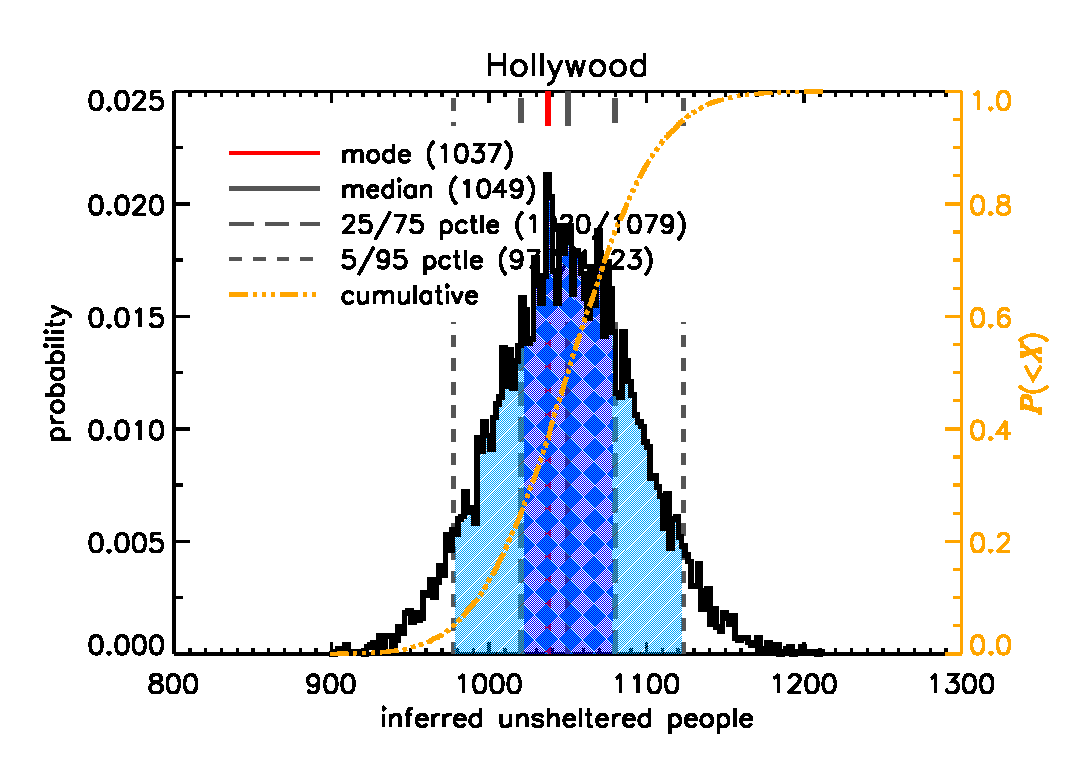
\includegraphics[width =\linewidth]{hWood/HollywoodDist}
	\caption{}
\end{figure}

\subsection{East Hollywood CoC}
\label{sec:eHo}

\begin{figure}[h]
	\centering
	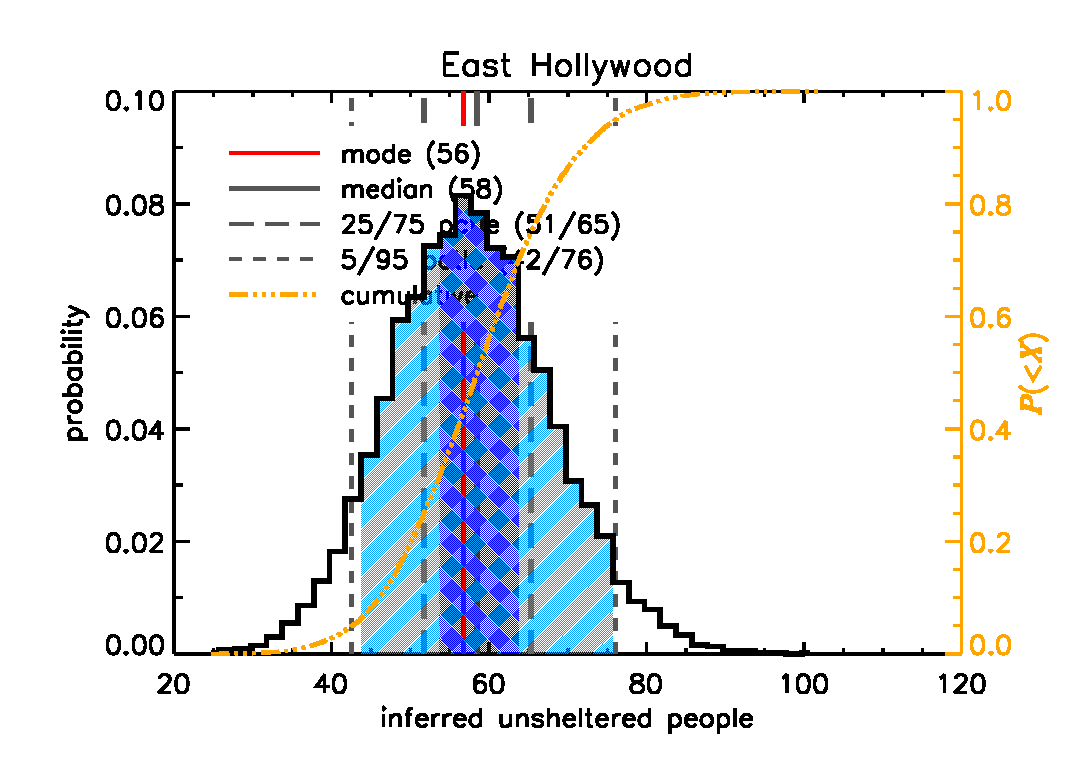
\includegraphics[width =\linewidth]{eHo/EastHollywoodDist}
	\caption{}
\end{figure}

\begin{figure*}[h]
	\centering
	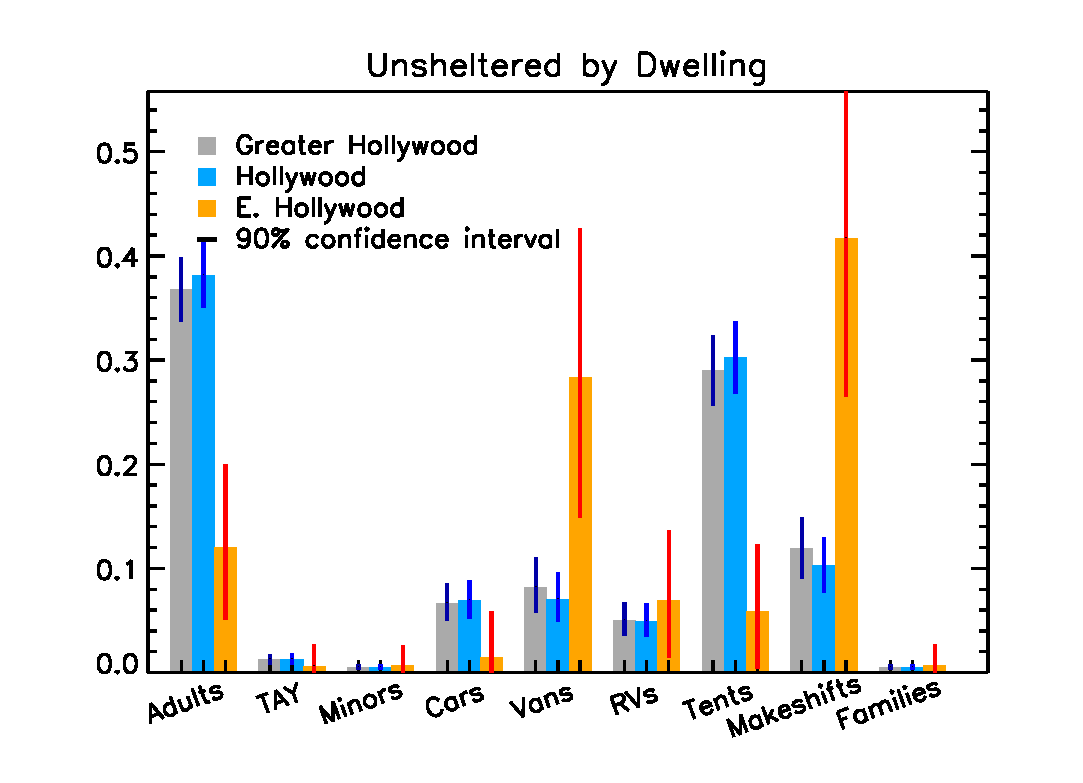
\includegraphics[width =\linewidth]{allTracts/allBreakdownBar}
	\caption{}
\end{figure*}

\subsection{Comparison to 2020}
\label{sec:comp}

\section{Discussion}
\label{sec:discussion}

We discuss these potential sources of systematic errors below.

\subsection{Null Entries and TAY}
\label{sec:nulls}

As stated in Section \ref{sec:training}, some (too few) tracts have unsheltered populations near zero, 
or at least are not observed to host any people or dwellings of a specific category. Such null entries 
are consistent with a range of non-zero values for the true population due to shot noise. As such, the 
Monte Carlo PDF reconstruction must allow them to take non-zero values based on an assumed background
rate. 
%This fact is immaterial 
%when the global category population is high, but such is not the case for TAY, unaccompanied 
%minors, and families. Treatment of null entries therefore affects estimates for those sub-populations,
%or defines their upper limits.

Ideally, that rate would be based on the variations in a category's counts (or count densities) in other, 
similar tracts defined by some independent criteria. While sufficient data from, e.g., the US Census 
may enable such an exercise, it is beyond the scope of this analysis. Instead, we base our noise floor 
on the number of counts of a given category expected if the total was evenly distributed across 
all tracts. That is:
\begin{equation}
	\sigma_{j,\,\rm min}^{2} = \frac{1}{39}\sum_{\rm tracts}n_{j},
\end{equation}
where $\sigma_{j}$ and $n_{j}$ are defined as in Equation \ref{eq:monte}.

This method works for any category, $j$, for which there is at least one individual/dwelling observed in any 
tract. However, for categories for which even this is not the case---unaccompanied minors and families, in the
case of Hollywood---we set $\sigma_{j, \rm min}$ to the lowest non-zero value of the other categories
(corresponding to TAY).

{\bfr State the bkg levels.}

{\it While we admit that such a treatment is 
somewhat arbitrary}, due to the intrinsically low levels of at least unsheltered unaccompanied minors 
and families, it does not significantly affect our CoC level estimates. It does affect TAY, however, and
as such, taken with the difficulty of disambiguating older TAY from younger adults, we caution against 
relying on the TAY estimates for anything beyond lower-limits.

\subsection{CVRTM Biases}
\label{sec:CVRTM}

Less easily handled are potential biases in the CVRTM demographic weights our \Count\ adopts.
Typically, specialized teams perform detailed interviews of people experiencing homelessness to update 
these weights in various geographic contexts. However, the cancellation of the official PIT count means
that this will not occur in 2021. As such, we are forced to rely on year-old estimates.

We present 

\subsubsection{Nulling the 2021 Result}
\label{sec:nullOut}

\subsubsection{Examining Past Variability}
\label{sec:pastValues}

\subsubsection{Relying on Smaller Geographies}
\label{sec:cdWts}

\subsubsection{Using External Data}
\label{sec:bidData}

The Hollywood Partnership---one of Hollywood's Business Improvement Districts (BIDs)---has performed
weekly visual scans of its footprint since spring 2019. These inspections tally unsheltered people and 
tents separately. As such, they can be used to bound the possible evolution of the CVRTM tent weight
between the official 2020 value and what it may be today.

{\bfr SECZ}

A lower-bound on the the weight can be derived by assuming that all of the tents captured by the BID's 
censuses were empty and all of their inhabitants visible. The weight would the be just the number of
people on the number of tents. If any of the tents were not empty, the true weight would be higher than
the inferred weight. Ergo, the BID/SECZ derived tent weight may reflect a {\it conservative} estimate 
which, when applied to the entire footprint, would produce something like a lower-bound on the 
tent contribution to the 2021 \Count.

{\bfr We'll use the BID counts outside the SEZ and find (tents+people)/tents for the past year. We'll
fit it and get a range of values for the night of the count. It's typically higher than 1.45 (thru last July,
at least), so we can just find the decline and peg it to 1.45.}

{\bfr Plot the trend; discuss it in terms of the 2020 value; see what it does; talk about why we don't
think most of the folks on foot in the SECZ are interlopers.}

\section{Summary}
\label{sec:summary}

\appendix

\section{Example Documents}

\begin{figure*}
	\centering
	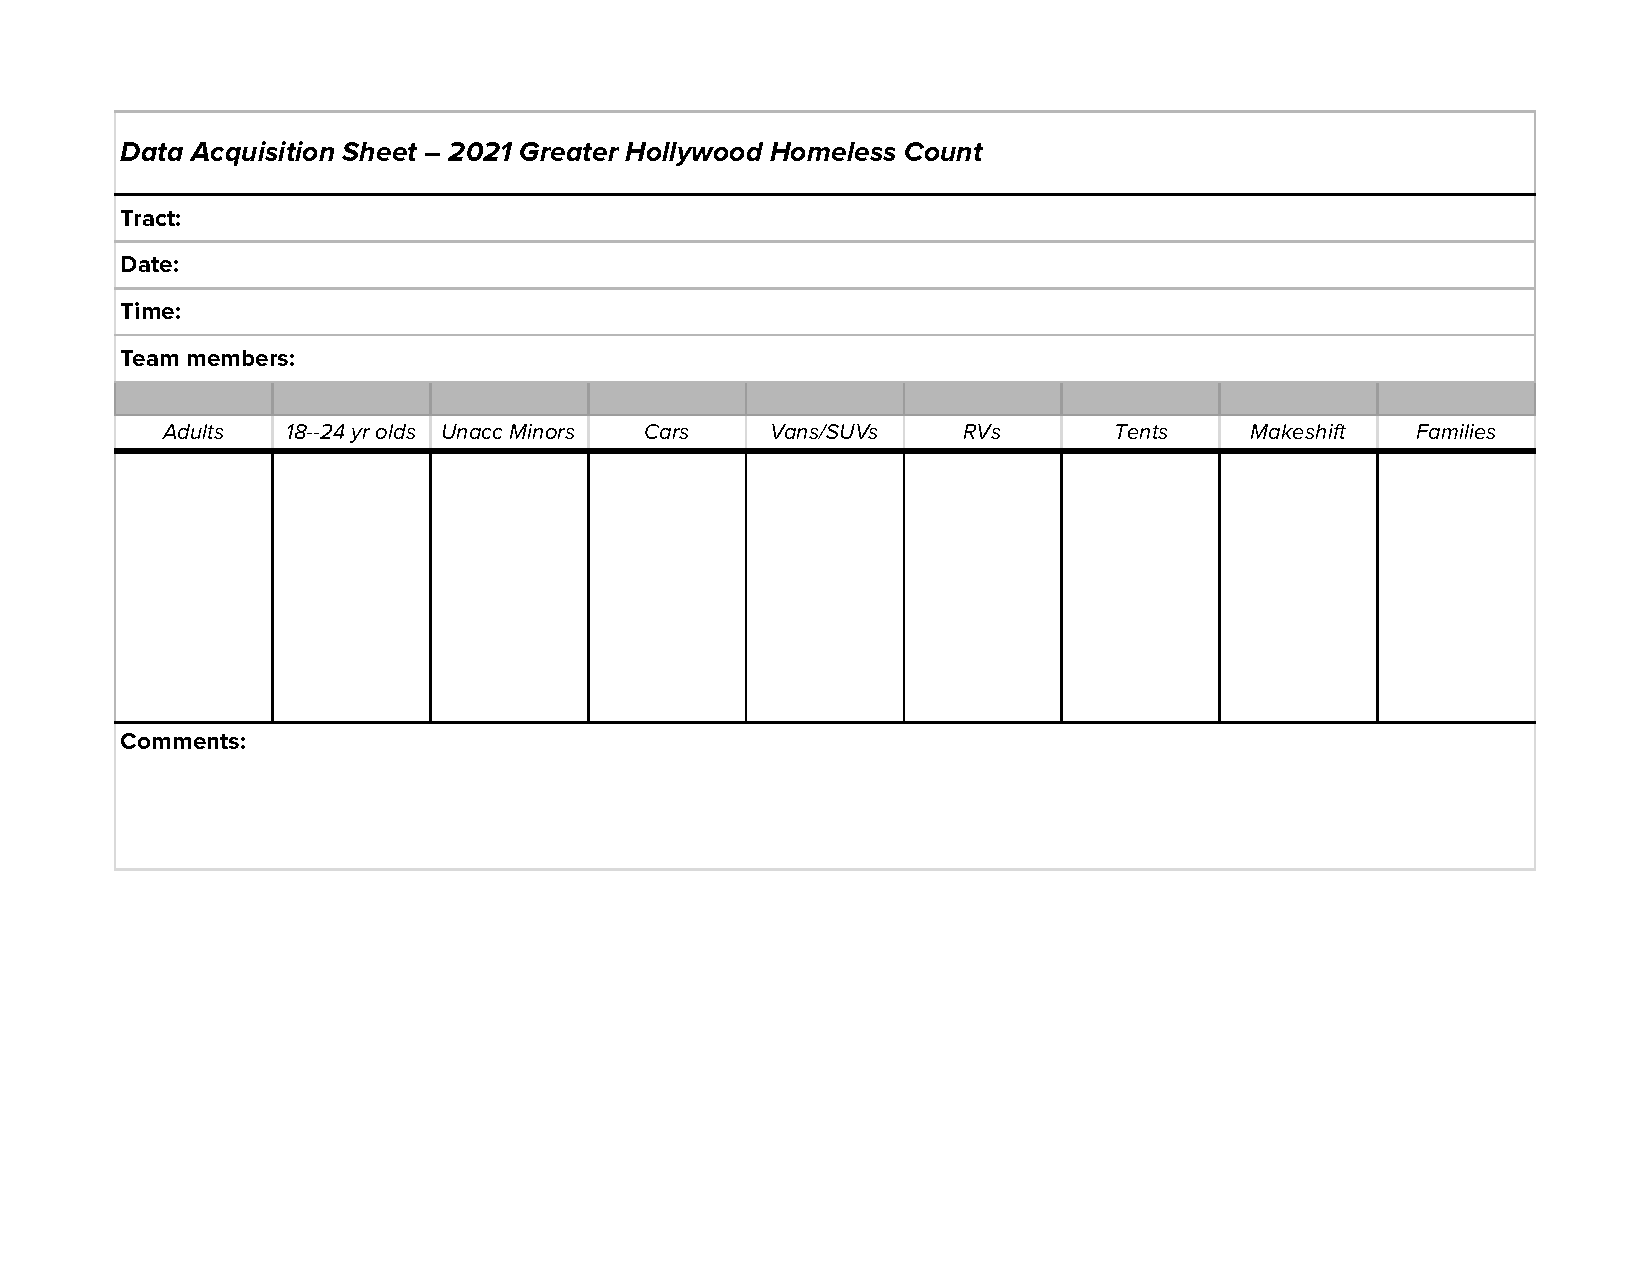
\includegraphics[width =\linewidth]{Hollywood2021CountDataSheet}
	\caption{Counter tally-sheet}
\end{figure*}

\begin{figure*}
	\centering
	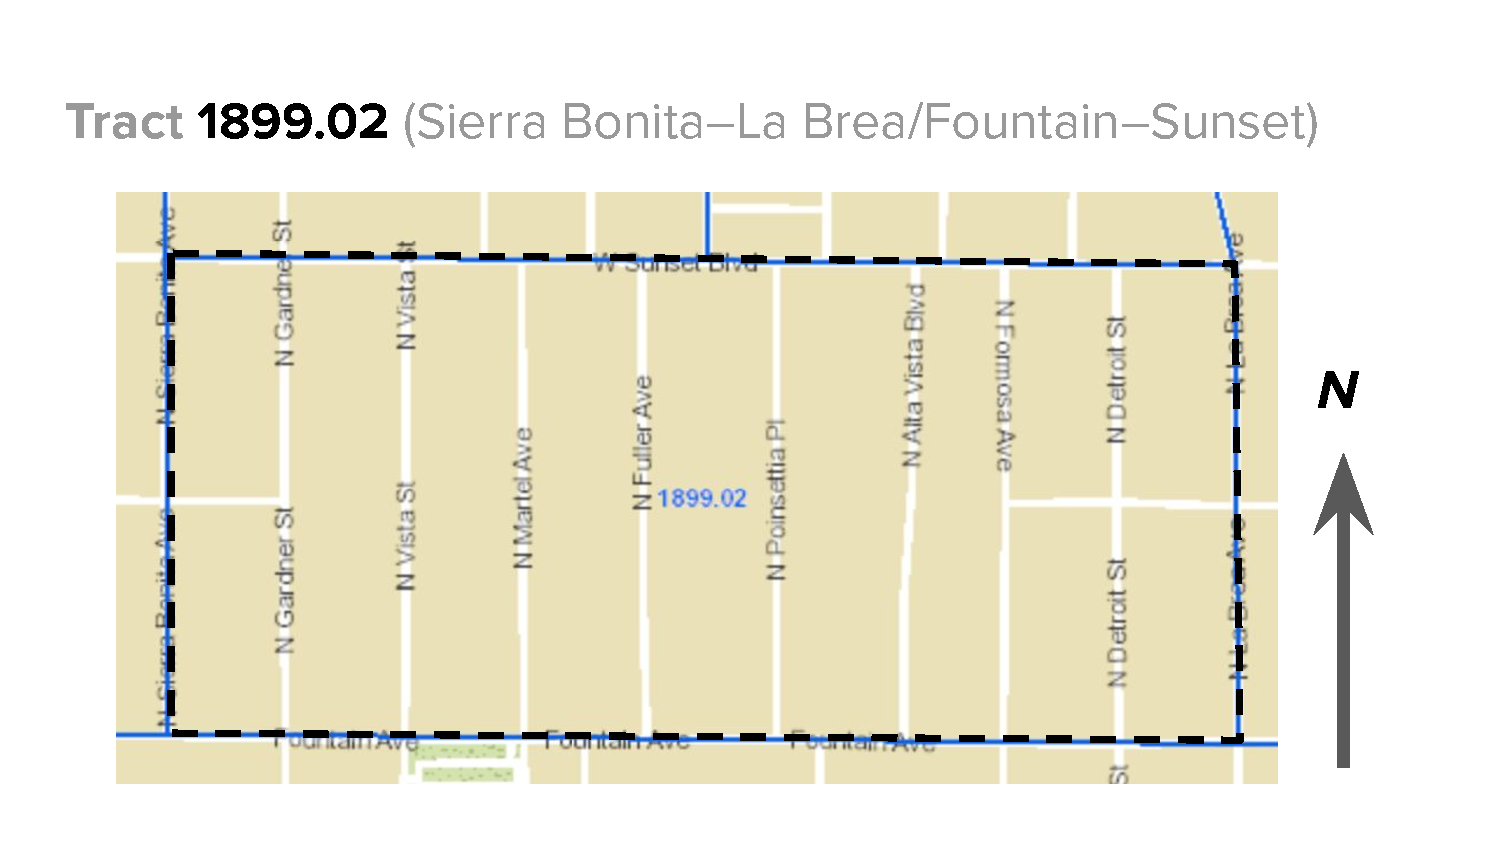
\includegraphics[width =\linewidth]{tractMap}
	\caption{Example Hollywood tract map.}
\end{figure*}

\begin{figure*}
	\centering
	\includegraphics[width =0.7\linewidth]{primerFront}
	\caption{Count primer {\bfr SCRUB EK'S NUMBER!}}
\end{figure*}

\section{Full Tract-level Results}

\end{document}  